\chapter{Diseño e implementación} % Main chapter title

\label{Chapter3} % Change X to a consecutive number; for referencing this chapter elsewhere, use \ref{ChapterX}

\definecolor{mygreen}{rgb}{0,0.6,0}
\definecolor{mygray}{rgb}{0.5,0.5,0.5}
\definecolor{mymauve}{rgb}{0.58,0,0.82}

%%%%%%%%%%%%%%%%%%%%%%%%%%%%%%%%%%%%%%%%%%%%%%%%%%%%%%%%%%%%%%%%%%%%%%%%%%%%%
% parámetros para configurar el formato del código en los entornos lstlisting
%%%%%%%%%%%%%%%%%%%%%%%%%%%%%%%%%%%%%%%%%%%%%%%%%%%%%%%%%%%%%%%%%%%%%%%%%%%%%
\lstset{ %
  backgroundcolor=\color{white},   % choose the background color; you must add \usepackage{color} or \usepackage{xcolor}
  basicstyle=\footnotesize,        % the size of the fonts that are used for the code
  breakatwhitespace=false,         % sets if automatic breaks should only happen at whitespace
  breaklines=true,                 % sets automatic line breaking
  captionpos=b,                    % sets the caption-position to bottom
  commentstyle=\color{mygreen},    % comment style
  deletekeywords={...},            % if you want to delete keywords from the given language
  %escapeinside={\%*}{*)},          % if you want to add LaTeX within your code
  %extendedchars=true,              % lets you use non-ASCII characters; for 8-bits encodings only, does not work with UTF-8
  %frame=single,	                % adds a frame around the code
  keepspaces=true,                 % keeps spaces in text, useful for keeping indentation of code (possibly needs columns=flexible)
  keywordstyle=\color{blue},       % keyword style
  language=[ANSI]C,                % the language of the code
  %otherkeywords={*,...},           % if you want to add more keywords to the set
  numbers=left,                    % where to put the line-numbers; possible values are (none, left, right)
  numbersep=5pt,                   % how far the line-numbers are from the code
  numberstyle=\tiny\color{mygray}, % the style that is used for the line-numbers
  rulecolor=\color{black},         % if not set, the frame-color may be changed on line-breaks within not-black text (e.g. comments (green here))
  showspaces=false,                % show spaces everywhere adding particular underscores; it overrides 'showstringspaces'
  showstringspaces=false,          % underline spaces within strings only
  showtabs=false,                  % show tabs within strings adding particular underscores
  stepnumber=1,                    % the step between two line-numbers. If it's 1, each line will be numbered
  stringstyle=\color{mymauve},     % string literal style
  tabsize=2,	                   % sets default tabsize to 2 spaces
  title=\lstname,                  % show the filename of files included with \lstinputlisting; also try caption instead of title
  morecomment=[s]{/*}{*/}
}
%----------------------------------------------------------------------------------------

\textit{ NOTA: ESTE CAPÍTULO SE ENCUENTRA EN CONSTRUCCIÓN.}

En este capítulo se detallan los componentes de software y hardware diseñados e implementados por el autor, su interrelación, y los criterios seguidos.

%----------------------------------------------------------------------------------------
%	SECTION 1
%----------------------------------------------------------------------------------------
\section{Arquitectura del sistema}

Para abordar el trabajo realizado, en esta sección se expone la arquitectura general del sistema embebido implementado, esquematizada en el diagrama de la figura \ref{fig:diagramaCompleto}, y luego, en las siguientes secciones, se detallan cada uno de los componentes de manera individual.

\begin{figure}[htbp]
	\centering
	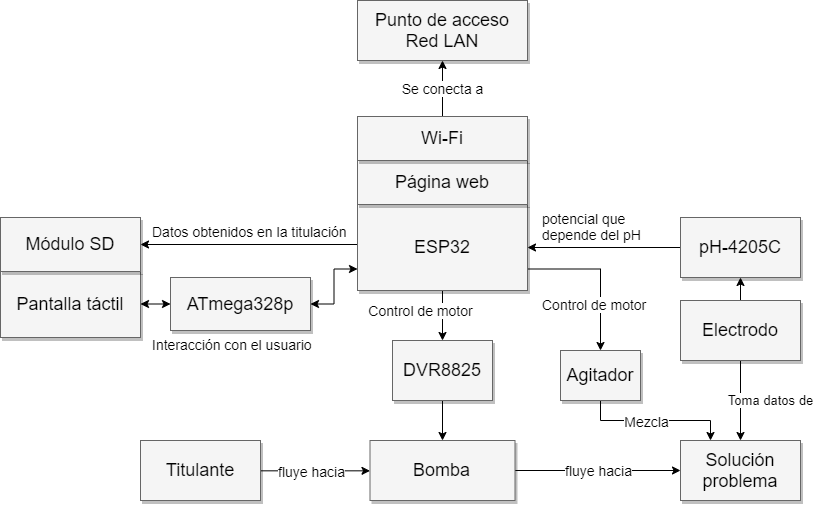
\includegraphics[width=1.0\textwidth]{./Figures/DiagramaBloquesCompleto.png}
	\caption{Diagrama en bloques del trabajo realizado.}
	\label{fig:diagramaCompleto}
\end{figure}

El componente principal del sistema es el ESP32, que tiene como función coordinar cada una de las partes intervinientes. A través de una comunicación del tipo UART, recibe las órdenes ingresadas a través de la pantalla táctil y  son procesadas por el ATmega328p, para realizar las configuraciones o funciones que solicite el usuario.

Dentro de las configuraciones, está la posibilidad de modificar el volumen de corte y de habilitar, o no, el agitador. El volumen de corte es la cantidad máxima de titulante que se utiliza durante la titulación. Cuando se alcanza ese valor, el proceso se detiene automáticamente. En cuanto a la habilitación del agitador, permite elegir si el mismo se activa o no al inicial la titulación.

Las funciones que ofrece el sistema son las de limpieza, calibración y titulación. El modo limpieza se utiliza para purgar la bomba previo al proceso de titulación y para eliminar los retos de titulante que quedan en las mangueras al finalizar el proceso. 

La calibración permite ajustar el valor leído por el ADC, en el cual se encuentra conectado el módulo pH4502C. Para llevarla a cabo, se hace uso de tres líquidos patrones, denominados \textit{buffers}, de pH 4, 7 y 10, respectivamente. Se debe realizar la calibración de manera periódica, ya que las propiedades del electrodo varían con el tiempo.

Una vez realizadas las configuraciones correspondientes, la limpieza y la calibración, es posible iniciar la titulación. Cuando esto sucede, el ESP activa  la bomba para que comience a inyectar el titulante en la muestra problema, y registra los valores de pH asociados, que obtiene desde el electrodo. En la pantalla se visualiza una curva del pH a lo largo del tiempo, y se ofrece la posibilidad de finalizar el proceso, mediante un botón, en el momento que el usuario lo desee. En caso contrario, el proceso finaliza al alcanzar el volumen de corte.

Una vez finalizado el proceso, el ESP32 calcula la derivada primera para cada valor de volumen y pH asociados, y, en base a ello, encuentra el valor de volumen inyectado en el punto final. Tanto este valor, como todos los valores registrados, se almacenan en la memoria SD, a través de una comunicación SPI con el módulo correspondiente, y en la página web, que se encuentra embebida en la memoria del ESP32. A través de una conexión de área local se puede acceder a esta página desde otro dispositivo y visualizar los resultados.

Para realizar las actividades mencionadas previamente, el ESP32 ejecuta tres tareas: la tarea encargada de la comunicación UART con el ATmega328p, que se aloja en el núcleo 0, y las tareas de medición del electrodo y de control de la bomba, que se alojan en el núcleo 1. Además, existe un controlador de eventos, que se ejecuta sobre el núcleo 0 cuando alguien accede a la página web.


%----------------------------------------------------------------------------------------
\section{Medición del electrodo}

La medición del electrodo es un módulo de software que tiene una tarea de FreeRTOS asociada. El objetivo de esta tarea es obtener el valor en mV que entrega el módulo pH-4502C y es ejecutada durante el proceso de calibración y el de titulación. En el código \ref{cod:tareaElectrodo} se muestra el pseudocódigo de la tarea de medición del electrodo. Al inicio de esta tarea se realiza la configuración del ADC utilizado, el cual se habilita con resolución 12 bits en el pin correspondiente al canal 6 del ADC número 1.

La lectura del valor del ADC se acumula en la variable sumaAdc durante las N iteraciones del bucle for. Cada una de estas iteraciones se realiza en un intervalo de 10 mS, y, al finalizar el bucle for, el valor total se divide por la cantidad de muestras realizadas, lo que permite promediar el valor leído y así reducir el ruido presente en la conversión, tal y como sugiere la página oficial del ESP32 \citep{WEBSITE:2}. Cabe destacar que el acceso a la variable valorAdc está protegido por una sección crítica, ya que resto de las tareas también pueden acceder a la variable cuando precisan calcular el valor de pH.

\begin{lstlisting}[label=cod:tareaElectrodo,caption=Pseudocódigo de la tarea de medición de pH.]
void tareaElectrodo (void *arg)
{
    //Configuracion de resolucion y pin del ADC
    configuracionADC(12 bits, pin);
    uint32_t sumaAdc = 0;

    while(true)
    {
    for (int i=0; i< N_MUESTRAS; i++)
    {
        sumaAdc = sumaAdc + lecturaADC(pin);  
        vTaskDelay(10 mS);
    } 
    inicioSeccionCritica(); 
    valorAdc = sumaAdc / N_MUESTRAS;
    finSeccionCritica();
    sumaAdc = 0;
    }
}
\end{lstlisting}

%----------------------------------------------------------------------------------------
\section{Control de la bomba}

El control de la bomba se realiza a través del \textit{driver} DVR8825, que maneja al motor paso a paso, y, mediante hardware, fue configurado con el \textit{microsteping} en 1/32. Esto significa que el motor debe realizar 6400 micropasos para producir un giro completo. Los pines de dirección y de paso están conectados a dos pines del ESP32. El pin de dirección fue configurado mediante software para producir el sentido de giro que permite desplazar el titulante desde su recipiente hasta el recipiente de la muestra. En cuanto al pin de paso, este es controlado por PWM, que genera una onda cuadrada de 10 KHz. Esto se traduce a una velocidad de 93,74 rpm en el eje del motor.

Las configuraciones de software mencionadas anteriormente se realizan al inicio la tarea de control de la bomba, en el bloque correspondiente a configuración de PWM del diagrama que muestra la figura \ref{fig:flujoBomba}.

Una vez realizadas las configuraciones, la tarea de control de la bomba tiene la posibilidad de ejecutar dos funciones según lo que decida el usuario a través de la pantalla táctil. Una de las opciones el el proceso de limpieza, en el cual simplemente se activa la bomba, es decir, se habilita el PWM que produce la onda cuadrada que llega al pin de paso del DVR8825 y genera el giro del motor. Este proceso se ejecuta hasta que el usuario decida detenerlo.

La otra función corresponde al proceso de titulación. El requerimiento TPA-ERS-01-REQ012 establece que es necesario inyectar 0,1 mL y luego realizar una espera de 5 segundos antes de realizar la medición de pH. Está cantidad de volumen se logran cuando el motor produce 11500 micropasos, lo que equivale a que el PWM esté activado durante 1150 ms, valor definido mediante la etiqueta T-CORTO. Además, el requerimiento contempla que, para cuando la variación de pH entre dos mediciones  es menor a 0,2, se puede inyectar 1 mL en lugar de 0,1 mL, por lo cual se define la etiqueta T-LARGO en 11500 ms. Esto es útil para agilizar el proceso, especialmente al inicio de la titulación, donde el pH varía de manera lenta a medida que se agrega volumen, como se mostró anteriormente en la figura \ref{fig:sigmoidea}. Las pruebas que permitieron llegar a estos valores son mencionadas en el capítulo \ref{Chapter4}.

\begin{figure}[htbp]
	\centering
	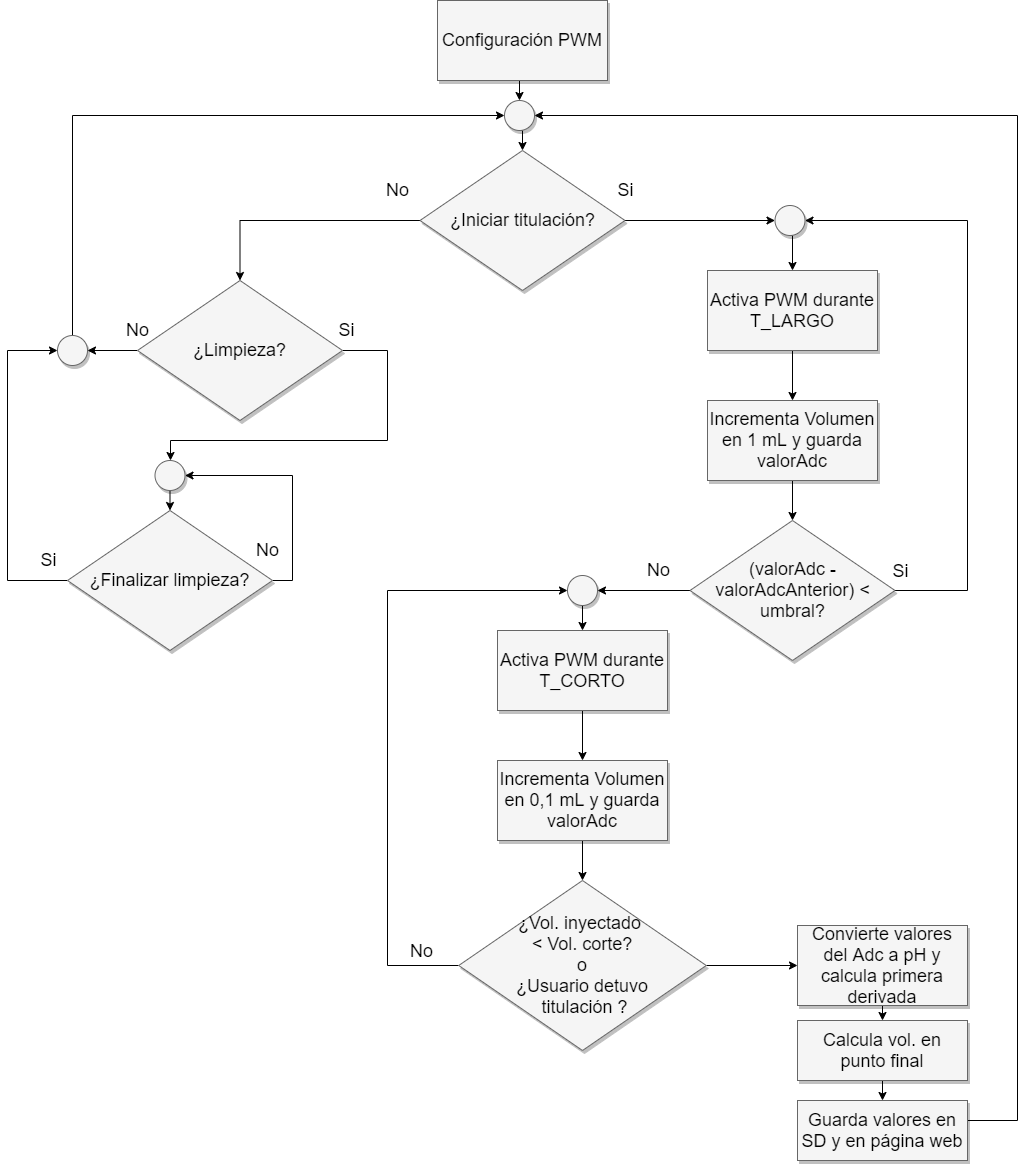
\includegraphics[width=1.0\textwidth]{./Figures/motorBomba.png}
	\caption{Diagrama de flujo de la tarea de control de la bomba.}
	\label{fig:flujoBomba}
\end{figure}

Ya definidas las configuraciones y los tiempos para cada cantidad del volumen, el proceso de titulación inicia con la activación del PWM que produce el giro de la bomba hasta alcanzar la cantidad de 1 mL de titulante inyectado. Llegado a este punto, se produce una espera de 5 segundos y luego, el valor leído por la tarea del electrodo se almacena en un arreglo, al igual que la cantidad de volumen acumulado. El proceso se repite hasta que la diferencia entre las dos ultimas mediciones del electrodo supere un umbral, equivalente a aproximadamente 0,2 pH. A partir de este momento, se modifica la cantidad de volumen inyectado a 0,1 mL, pero el resto del procedimiento es el mismo. Una vez alcanzado el volumen de corte, o si el usuario presiona el boton de finalizar, la bomba de detiene y se procede a una función que calcula el valor de pH para cada valor almacenado en el arreglo de mediciones del electrodo. Luego, se calcula el valor de la primera derivada del pH respecto al volumen para cada uno de los valores del arreglo y se determina el volumen en el punto final en base al valor máximo de la primera derivada. Todos los valores son almacenados en la memoria SD y en la página web para que el usuario pueda tener acceso, el el valor de volumen en el punto final es mostrado en la pantalla.


%----------------------------------------------------------------------------------------
\section{Interfaz de usuario}

La interfaz de usuario permite el acceso a todas las configuraciones y funciones que presenta el titulador. Está implementada a través de una pantalla táctil que permite navegar por un menú de diferentes pantallas, que fueron implementadas mediante la máquina de estados de la figura \ref{fig:MEFmenu}.

La máquina de estados se ejecuta en el ATMega328p y cada estado tiene una pantalla gráfica asociada con botones táctiles que permiten navegar entre las diferentes opciones. Por ejemplo, desde el menú inicial se puede acceder al menú de titulación a través del botón TITULAR.

\begin{figure}[htbp]
	\centering
	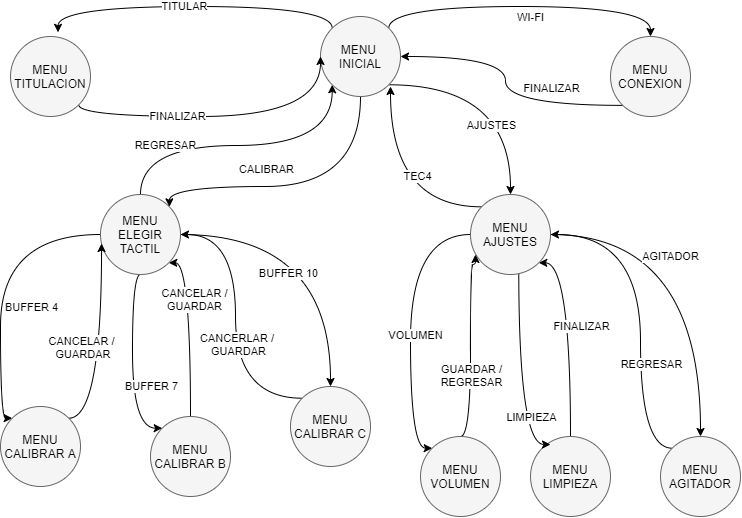
\includegraphics[width=1.0\textwidth]{./Figures/MEFmenu.png}
	\caption{Máquina de estados del menú de usuario.}
	\label{fig:MEFmenu}
\end{figure}

A continuación se listan las características de cada uno de los estados:

\begin{itemize}
\item Menú inicial: es el estado en el cual se ingresa cuando se inicia el programa. Desde aquí se puede acceder a la calibración, a la titulación, al menú de ajustes y al menú de conexión.
\item Menú elegir \textit{buffer}: se utiliza para elegir el \textit{buffer} (patrón) con el cual se desea calibrar. Para completar el proceso de calibración de manera correcta, se debe ingresar en cada uno de los tres \textit{buffers}. Al presionar REGRESAR se envía por UART que el proceso de calibración finalizó para que el ESP32 actualice la función correspondiente al calculo del valor de pH.
\item Menú calibrar A: es el estado en el cual se calibra usando el \textit{buffer} de pH 4. En este estado el ATmega328p se comunica con el ESP32 para solicitarle el valor actual de pH. Este valor sirve como referencia para que el usuario presione GUARDAR una vez que la lectura sea estable. Al presionar GUARDAR, se envía la confirmación al ESP32 para que actualice el valor correspondiente al \textit{buffer} de pH 4, y se regresa al menú de elegir \textit{buffer}. En caso de presionar regresar, vuelve al menú pero sin enviar la confirmación al ESP32.
\item Menú calibrar B: es el estado en el cual se calibra usando el \textit{buffer} de pH 7, y sigue el mismo procedimiento que el menú calibrar A.
\item Menú calibrar C: es el estado en el cual se calibra usando el \textit{buffer} de pH 10, y sigue el mismo procedimiento que el menú calibrar A.
\item Menú titulación: es el estado en el cual se realiza el proceso de titulación, por ende, se envía un comando al ESP32 para que se ejecute la función de titulación dentro de la tarea de la bomba.
\item Menú ajustes: es el estado que permite acceder a varias configuraciones.
\item Menú volumen: es el estado que permite seleccionar el volumen de corte. Cuando se ingresa a este, se envía un comando al ESP32 para consultar el volumen de corte actual y mostrarlo en pantalla. Mediante un botón + y otro botón - se puede variar de a 1 mL este valor. Luego al presionar GUARDAR se envía el nuevo valor al ESP32, mientras que si se presionar REGRESAR vuelve al menú anterior sin hacer cambios.
\item Menú limpieza: es el estado que permite purgar o limpiar las mangueras de la bomba.  Aquí se envía un comando al ESP32 para que ejecute la función de limpieza dentro de la tarea de la bomba.
\item Menú agitador: es el estado que permite habilitar o deshabilitar el uso del agitador. Tiene los botones ON y OFF que enviarán al ESP32 el comando correspondiente para activar o desactivar el agitador respectivamente.
\item Menú conexión: es el estado que permitirá acceder a configuraciones de la conexión Wi-Fi. Actualmente muestra la pantalla correspondiente pero no ejecuta ninguna acción.
\end{itemize}

Como se mencionó anteriormente, la máquina de estados funciona dentro del ATmega328p y en algunos estados se produce una comunicación del tipo UART con el ESP32 para el intercambio de la información necesaria. Esta comunicación se realiza mediante comandos que representan determinadas acciones, tal y como muestra la tabla


\begin{table}[h]
	\centering
	\caption[Comandos UART]{Comandos utilizados en la comunicación UART entre el ESP32 y el ATmega328p.}
	\begin{tabular}{l c c c }    
		\toprule
		\textbf{Comando} & \textbf{Valor asociado}	&    \textbf{Acción } \\
		\midrule
		A	&  &  		 \\
		B	&  &  		 \\		
		C	&  &  		 \\	
		D	&  &  		 \\	
		E	&  &  		 \\	
		F	&  &  		 \\		
		G	&  &  		 \\	
		H	&  &  		 \\	
		I	&  &  		 \\	
		J	&  &  		 \\		
		K	&  &  		 \\	
		L	&  &  		 \\	
		M	&  &  		 \\	
		N	&  &  		 \\		
		O	&  &  		 \\	
		P	&  &  		 \\	
		Q	&  &  		 \\	
		\bottomrule
		\hline
	\end{tabular}
	\label{tab:titComerciales}
\end{table}


%----------------------------------------------------------------------------------------
\section{Proceso de calibración}

%----------------------------------------------------------------------------------------
\section{Almacenamiento de datos}

%----------------------------------------------------------------------------------------
\section{Servidor web}

%----------------------------------------------------------------------------------------
\section{Esquemáticos y PCB}
